\chapter{\ifproject%
      \ifenglish Experimentation and Results\else การทดลองและผลลัพธ์\fi
  \else%
      \ifenglish System Evaluation\else การประเมินระบบ\fi
  \fi}



% \section{\ifenglish put the name here \else การสำรวจความคิดเห็นต่อเกมสยองขวัญ\fi}
% จากผลสำรวจกลุ่มเป้าหมายทั้งหมด 47 คน ได้ผลสรุปดังนี้
% \begin{itemize}
%     \item สาเหตุที่ผู้เล่นนั้น ไม่สามารถเล่นเกมจนจบได้นั้น คือ อันดับ 1 ไม่มีเวลาเล่น คิดเป็น 74.5$\%$, อันดับ 2 ไม่มีคนเล่นด้วย คิดเป็น 53.2$\%$, และอันดับ 3 คู่ร่วม คือ เนื้อเรื่องไม่มีความน่าสนใจ และ มีเกมอื่นที่น่าสนใจมากกว่า คิดเป็น 18.3$\%$
%     \item เกมแนวสยองขวัญควรมีอะไรบ้าง คือ อันดับ 1 มีฉากนองเลือด คิดเป็น 85.1$\%$, อันดับ 2 มีบรรยากาศที่ดูอึดอัด คิดเป็น 76.6$\%$, และอันดับ 3 ความมืด คิดเป็น 74.5$\%$
%     \item สิ่งที่ไม่ถูกใจในเกมสยองขวัญคือ มีความยากในการเล่นสูงเกินไป มีความซ้ำซากจำเจ ต่อสู้กับผีไม่ได้ และมีฉาก jump scare มากเกินไป
% \end{itemize}
% \begin{figure}[h]
%     \centering
%     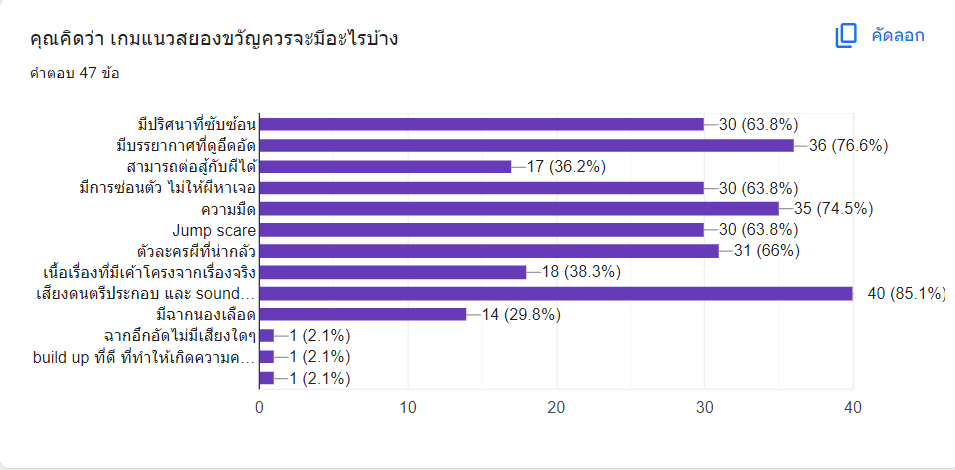
\includegraphics[width=\textwidth]{Images/Screenshot 2023-10-06 192027.png}
%     \caption{ภาพผลสำรวจความคิดเห็นที่มีต่อเกมสยองขวัญ}\label{Empatize}
% \end{figure}
% \section{\ifenglish put the name here \else การวางแผนการประเมินผลสัมฤทธิ์ของโปรเจค\fi}
% \begin{enumerate}
%     \item นำ prototype มาทดสอบกับกลุ่มผู้ใช้งาน โดยให้เวลาในการทดสอบของแต่ละคน 15 นาที โดยใช้อุปกรณ์ที่เราได้จัดเตรียมไว้
%     \item สอบถามปัญหา จากการใช้งาน prototype
%     \item นำแบบทดสอบให้ทำ หลังการทดสอบ โดยมีเนื้อหาใจความดังนี้
%     \begin{itemize}
%         \item ท่านให้ความน่ากลัวของเกมนี้ อยู่ในระดับไหน 0-10 โดยที่ 0 คือ ไม่เห็นน่ากลัวเลย, 3 คือ น่ากลัวนิดๆหน่อยๆ, 5 คือ ก็น่ากลัวนะ, 7 คือ น่ากลัวมากๆ, และ 10 คือ จะน่ากลัวไปไหน
%         \item ท่านให้ความสนุกอยู่ระดับ 0 - 10 โดยที่ 0 คือ ไม่สนุกเลย, 3 คือ สนุกนิดหน่อย, 5 คือ สนุกปานกลางๆ, 7 คือ สนุกมาก, และ 10 คือ สนุกที่สุด
%         \item มีเนื้อเรื่องส่วนใด ที่ท่านชอบมากที่สุด อธิบาย
%     \end{itemize}
% \end{enumerate}

\section{\ifenglish put the name here\else วัตถุประสงค์ของการทดสอบ\fi}
\begin{enumerate}
    \item ทดสอบว่าผู้เล่นนั้นได้รับความสนุกในด้านความน่ากลัว
    \item ผู้เล่นได้รับรู้เนื้อเรื่องของเกมที่ผู้แต่งจัดทำขึ้น
    \item ฉากและตัวละครที่ผู้จัดทำเลือกมามีความสวยงาม และ สามารถสร้างบรรยากาศที่น่ากลัวได้
    \item ผู้เล่นได้ทดลองเล่นเกมและทดลองระบบต่างๆ ภายในเกม
\end{enumerate}

\section{ขั้นตอนและวิธีการทดสอบ}
ผู้พัฒนาได้ทำการทดสอบกับผู้เล่นจำนวน 11 คน โดยผู้ทดสอบคือบุคคลที่มีความชื่นชอบในการเล่นเกม และผู้ทดสอบต้องมีอายุ 18 ปีขึ้นไป โดยแบ่งการทดสอบเป็น 2 กรณี
\begin{enumerate}
    \item กรณีแบบออนไลน์
          \begin{enumerate}
              \item ผู้เล่นทำการเปิดโปรแกรม Discord จากนั้นทำการแชร์หน้าจอและทำการเล่นเกมจนสิ้นสุด
              \item ผู้พัฒนาทำการเฝ้าดูพฤติกรรมของผู้เล่นที่มีต่อตัวเกม
              \item หลังจากผู้เล่นทำการเล่นเกมจนสิ้นสุด ผู้เล่นทำแบบทดสอบที่เราได้ตระเตรียมไว้
          \end{enumerate}
    \item กรณีแบบออนไซต์
          \begin{enumerate}
              \item ผู้เล่นทำการเล่นเกมจนสิ้นสุด
              \item ผู้พัฒนาทำการเฝ้าดูพฤติกรรมของผู้เล่นที่มีต่อตัวเกม
              \item หลังจากผู้เล่นทำการเล่นเกมจนสิ้นสุด ผู้เล่นทำแบบทดสอบที่เราได้ตระเตรียมไว้
          \end{enumerate}
\end{enumerate}

\section{\ifenglish put the name here \else ผลการทดสอบผลสัมฤทธิ์ของผู้เข้าร่วม\fi}
จากการทดสอบกับผู้เล่นจำนวน 11 คน โดยมีผลการทดสอบเป็นดังนี้

\begin{enumerate}
    \item หลังจากผู้เล่นทำการเล่นเกมจนเสร็จสิ้นนั้น คิดว่าเกมมีความยากง่ายเพียงใด 50$\%$ ของผู้เล่นบอกว่า เกมนั้นมีความยากระดับปานกลาง ไม่ยากและก็ไม่ง่าย 30$\%$ ของผู้เล่นบอกว่า เกมนั้นมีความยากต่อการเล่น และ 20$\%$ ของผู้เล่นบอกว่า เกมนั้นมีความง่าย ดังรูปที่ 4.1
    \begin{figure}
        \centering
        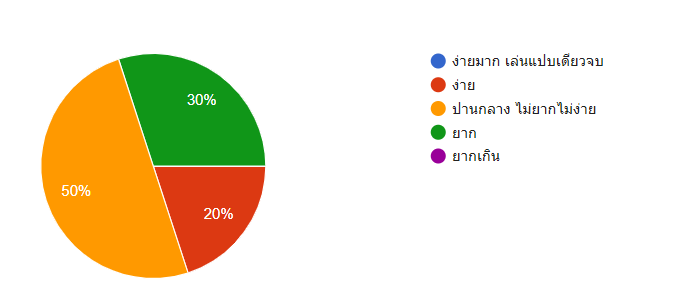
\includegraphics[width=0.8\textwidth, height=0.20\textheight]{Images/Graph difficult.png}
        \caption[การฟแสดงผลการทดสอบความยากง่ายของเกม]{การฟแสดงผลการทดสอบความยากง่ายของเกม}
    \end{figure}
    \item ระบบ Sanity ส่งผลต่ออุปสรรคในการเล่นเพียงใด 45.5$\%$ ของผู้เล่นบอกว่า ระบบ Sanity นั้น เป็นอุปสรรคต่อผู้เล่นปานกลาง 36.4$\%$ ของผู้เล่นบอกว่า ระบบ Sanity นั้น เป็นอุปสรรคต่อผู้เล่นมาก และ 18.2$\%$ ของผู้เล่นบอกว่า ระบบ Sanity นั้น เป็นอุปสรรคต่อผู้เล่นน้อย ดังรูปที่ 4.2
    \begin{figure}
        \centering
        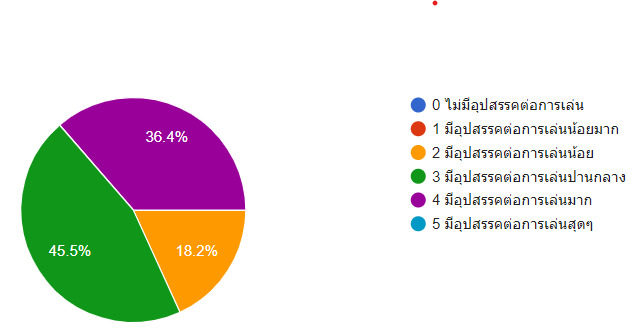
\includegraphics[width=0.8\textwidth, height=0.20\textheight]{Images/Graph Sanity.png}
        \caption[กราฟแสดงผลการทดสอบระบบ Sanity ส่งผลต่ออุปสรรคในการเล่นเพียงใด]{กราฟแสดงผลการทดสอบระบบ Sanity ส่งผลต่ออุปสรรคในการเล่นเพียงใด}
    \end{figure}
    \item ความรู้สึกหลังเล่น ความน่ากลัวของเกม 54.5$\%$ ของผู้เล่นบอกว่า เกมมีความน่ากลัวน้อย 36.4$\%$ ของผู้เล่นบอกว่า เกมมีความน่ากลัวปานกลาง และ 9.1$\%$ ของผู้เล่นบอกว่า เกมมีความน่ากลัวมากที่สุด ดังรูปที่ 4.3
    \begin{figure}
        \centering
        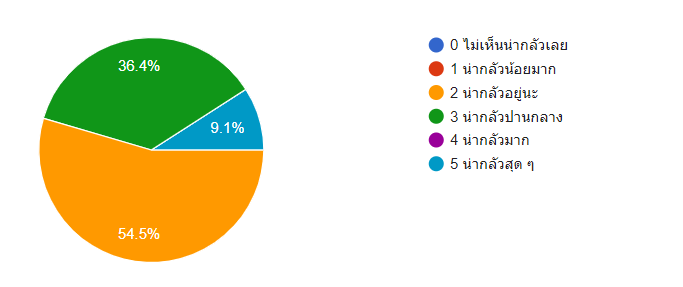
\includegraphics[width=0.8\textwidth, height=0.20\textheight]{Images/Graph Fear Level.png}
        \caption[กราฟแสดงผลการทดสอบความรู้สึกหลังเล่น ความน่ากลัวของเกม]{กราฟแสดงผลการทดสอบความรู้สึกหลังเล่น ความน่ากลัวของเกม}
    \end{figure}
    \item ความรู้สึกหลังเล่น ความกดดันของเกม 45.5$\%$ ของผู้เล่นบอกว่า เกมมีความกดดันปานกลาง 18.2$\%$ ของผู้เล่นบอกว่า เกมมีความกดดันมาก 18.2$\%$ ของผู้เล่นบอกว่า เกมมีความกดดันน้อย และ 18.2$\%$ ของผู้เล่นบอกว่า เกมมีความกดดันน้อยมาก ดังรูปที่ 4.4
    \begin{figure}
        \centering
        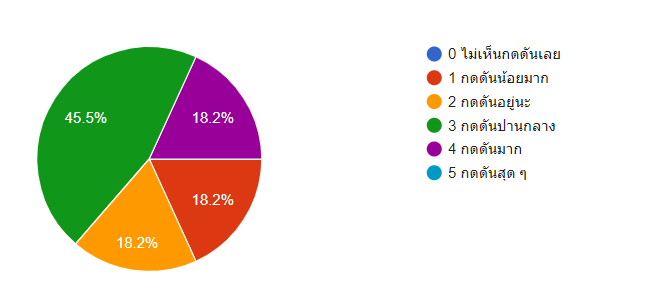
\includegraphics[width=0.8\textwidth, height=0.20\textheight]{Images/Graph Thresh Level.png}
        \caption[กราฟแสดงผลการทดสอบความรู้สึกหลังเล่น ความกดดันของเกม]{กราฟแสดงผลการทดสอบความรู้สึกหลังเล่น ความกดดันของเกม}
    \end{figure}
    \item เสียงประกอบของเกม 63.6$\%$ ของผู้เล่นบอกว่า เสียงประกอบเข้ากับสถานการณ์มาก 27.3$\%$ ของผู้เล่นบอกว่า เสียงประกอบเข้ากับสถานการณ์ปานกลาง และ 9.1$\%$ ของผู้เล่นบอกว่า เสียงประกอบเข้ากับสถานการณ์น้อยมาก ดังรูปที่ 4.5
    \begin{figure}
        \centering
        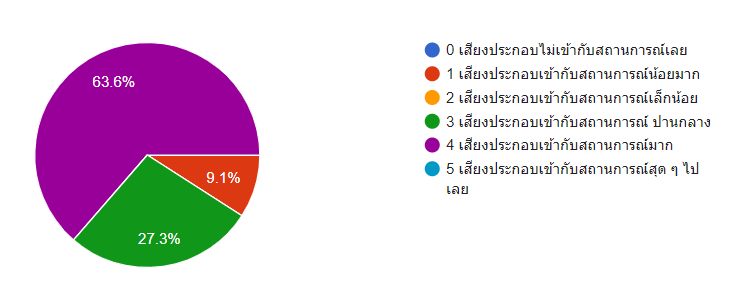
\includegraphics[width=0.8\textwidth, height=0.20\textheight]{Images/Graph Sounds.png}
        \caption[กราฟแสดงผลการทดสอบเสียงประกอบของเกม]{กราฟแสดงผลการทดสอบเสียงประกอบของเกม}
    \end{figure}
    \item ความเข้ากันของตัวละครหลักและฉาก 45.5$\%$ ของผู้เล่นบอกว่า ตัวละครเข้ากับฉากมาก 27.3$\%$ ของผู้เล่นบอกว่า ตัวละครเข้ากับฉากปานกลาง 18.2$\%$ ของผู้เล่นบอกว่า ตัวละครเข้ากับฉากเล็กน้อย และ 9.1$\%$ ของผู้เล่นบอกว่า ตัวละครเข้ากับฉากมากที่สุด ดังรูปที่ 4.6
    \begin{figure}
        \centering
        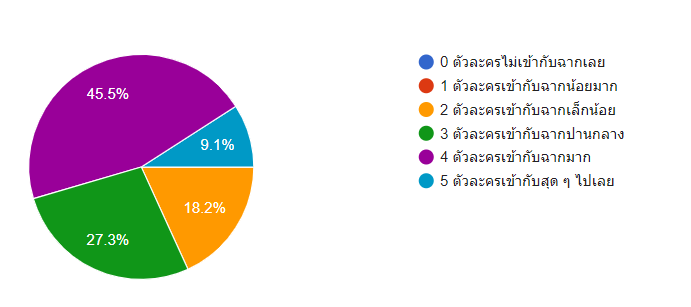
\includegraphics[width=0.8\textwidth, height=0.20\textheight]{Images/Graph Main Character.png}
        \caption[กราฟแสดงผลการทดสอบความเข้ากันของตัวละครหลักและฉาก]{กราฟแสดงผลการทดสอบความเข้ากันของตัวละครหลักและฉาก}
    \end{figure}
    \item ความเข้ากันของตัวละครแพรวและฉาก 45.5$\%$ ของผู้เล่นบอกว่า ตัวละครเข้ากับฉากปานกลาง 36.4$\%$ ของผู้เล่นบอกว่า ตัวละครเข้ากับฉากมาก 9.1$\%$ ของผู้เล่นบอกว่า ตัวละครเข้ากับฉากมากที่สุด และ 9.1$\%$ ของผู้เล่นบอกว่า ตัวละครเข้ากับฉากเล็กน้อย ดังรูปที่ 4.7
    \begin{figure}
        \centering
        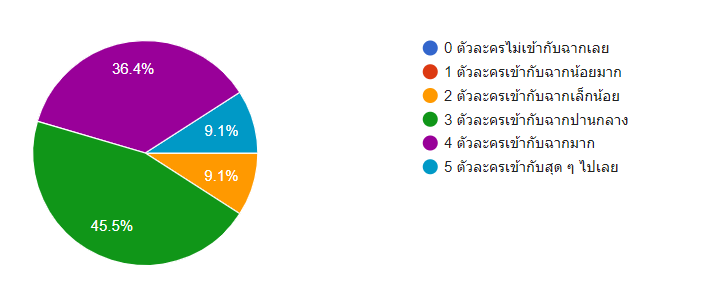
\includegraphics[width=0.8\textwidth, height=0.20\textheight]{Images/Graph Preaw Character.png}
        \caption[กราฟแสดงผลการทดสอบความเข้ากันของตัวละครแพรวและฉาก]{กราฟแสดงผลการทดสอบความเข้ากันของตัวละครแพรวและฉาก}
    \end{figure}
    \item ความเข้ากันของตัวละครศัตรูและฉาก 36.4$\%$ ของผู้เล่นบอกว่า ตัวละครเข้ากับฉากมากที่สุด 27.3$\%$ ของผู้เล่นบอกว่า ตัวละครเข้ากับฉากมาก 27.3$\%$ ของผู้เล่นบอกว่า ตัวละครเข้ากับฉากปานกลาง และ 9.1$\%$ ของผู้เล่นบอกว่า ตัวละครเข้ากับฉากน้อยมาก ดังรูปที่ 4.8
    \begin{figure}
        \centering
        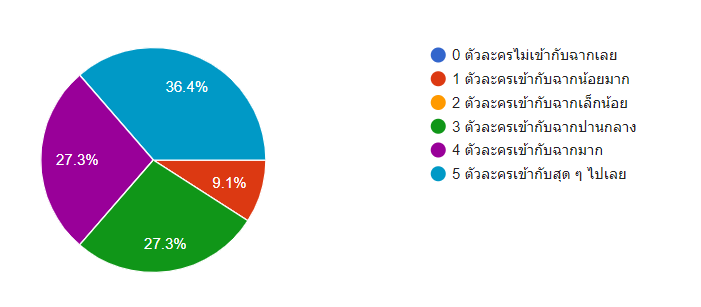
\includegraphics[width=0.8\textwidth, height=0.20\textheight]{Images/Graph Enemy Character.png}
        \caption[กราฟแสดงผลการทดสอบความเข้ากันของตัวละครศัตรูและฉาก]{กราฟแสดงผลการทดสอบความเข้ากันของตัวละครศัตรูและฉาก}
    \end{figure}
    \item ความสวยงามของฉากโรงเรียนตอนกลางวัน 54.5$\%$ ของผู้เล่นบอกว่า ฉากมีความสวยงามปานกลาง 36.4$\%$ ของผู้เล่นบอกว่า ฉากมีความสวยงามมาก และ 9.1$\%$ ของผู้เล่นบอกว่า ฉากมีความสวยงามน้อย ดังรูปที่ 4.9
    \begin{figure}
        \centering
        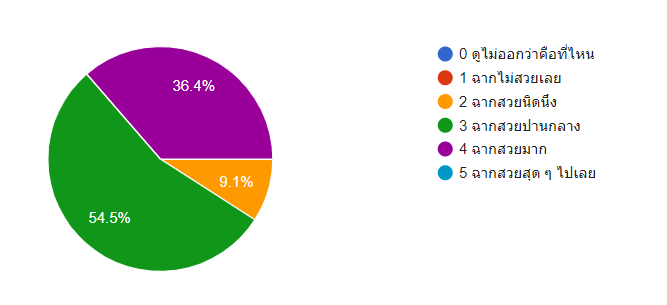
\includegraphics[width=0.8\textwidth, height=0.20\textheight]{Images/Graph School Day.png}
        \caption[กราฟแสดงผลการทดสอบความสวยงามของฉากโรงเรียนตอนกลางวัน]{กราฟแสดงผลการทดสอบความสวยงามของฉากโรงเรียนตอนกลางวัน}
    \end{figure}
    \item ความสวยงามของฉากโรงพยาบาล 54.5$\%$ ของผู้เล่นบอกว่า ฉากมีความสวยงามปานกลาง 18.2$\%$ ของผู้เล่นบอกว่า ฉากมีความสวยงามมาก 18.2$\%$ ของผู้เล่นบอกว่า ฉากมีความสวยงามน้อย และ 9.1$\%$ ของผู้เล่นบอกว่า ฉากมีความสวยงามมากที่สุด ดังรูปที่ 4.10
    \begin{figure}
        \centering
        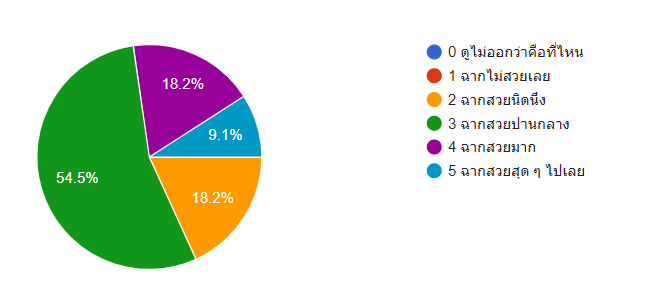
\includegraphics[width=0.8\textwidth, height=0.20\textheight]{Images/Graph Hospital.png}
        \caption[กราฟแสดงผลการทดสอบความสวยงามของฉากโรงพยาบาล]{กราฟแสดงผลการทดสอบความสวยงามของฉากโรงพยาบาล}
    \end{figure}
    \item ความสวยงามของฉากบ้านของแพรว 36.4$\%$ ของผู้เล่นบอกว่า ฉากมีความสวยงามมาก 36.4$\%$ ของผู้เล่นบอกว่า ฉากมีความสวยงามปานกลาง 18.2$\%$ ของผู้เล่นบอกว่า ฉากมีความสวยงามน้อย และ 9.1$\%$ ของผู้เล่นบอกว่า ฉากมีความสวยงามมากที่สุด ดังรูปที่ 4.11
    \begin{figure}
        \centering
        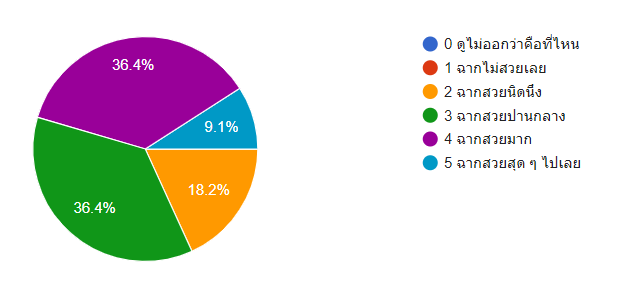
\includegraphics[width=0.8\textwidth, height=0.20\textheight]{Images/Graph Home.png}
        \caption[กราฟแสดงผลการทดสอบความสวยงามของฉากบ้านของแพรว]{กราฟแสดงผลการทดสอบความสวยงามของฉากบ้านของแพรว}
    \end{figure}
    \item ความสวยงามของฉากโรงเรียนตอนกลางคืน 45.5$\%$ ของผู้เล่นบอกว่า ฉากมีความสวยงามปานกลาง 27.3$\%$ ของผู้เล่นบอกว่า ฉากมีความสวยงามมาก 9.1$\%$ ของผู้เล่นบอกว่า ฉากมีความสวยงามมากที่สุด 9.1$\%$ ของผู้เล่นบอกว่า ฉากมีความสวยงามน้อย และ 9.1$\%$ ของผู้เล่นบอกว่า ดูไม่ออกว่าคืออะไร ดังรูปที่ 4.12
    \begin{figure}
        \centering
        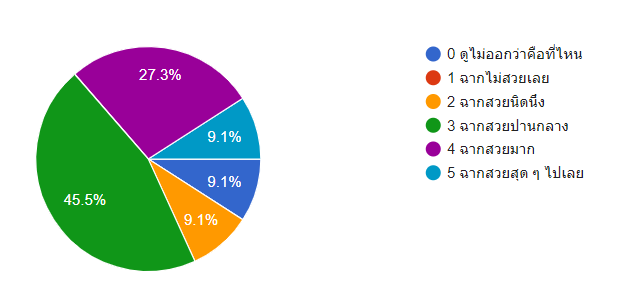
\includegraphics[width=0.8\textwidth, height=0.20\textheight]{Images/Graph School Night.png}
        \caption[กราฟแสดงผลการทดสอบความสวยงามของฉากโรงเรียนตอนกลางคืน]{กราฟแสดงผลการทดสอบความสวยงามของฉากโรงเรียนตอนกลางคืน}
    \end{figure}
\end{enumerate}

\section{\ifenglish put the name here\else สรุปผลการทดสอบผลสัมฤทธิ์\fi}
จากการประเมินผลสัมฤทธิ์ในการนำเกม Attention please: 3D side scrolling horror game ไปให้ผู้เล่นใช้จริง พบว่า ผู้เล่นได้รับความบันเทิงในเชิงของแนวสยองขวัญ และความสนุก คิดเป็น 50$\%$ ของผู้เล่น ที่ให้ความรู้สึกน่ากลัวและกดดันหลังเล่นของเรา
